%! TEX root = ../listas_completas.tex
\section{Lista 3}
\subsection{Questão 1}
Analisando a figura abaixo e considerando que entre o cilindro ``s'' e a
superfície não tenha deslizamento, encontre a massa equivalente para o sistema;
considerando como referência o cilindro s.

\begin{figure}[ht]
    \centering
    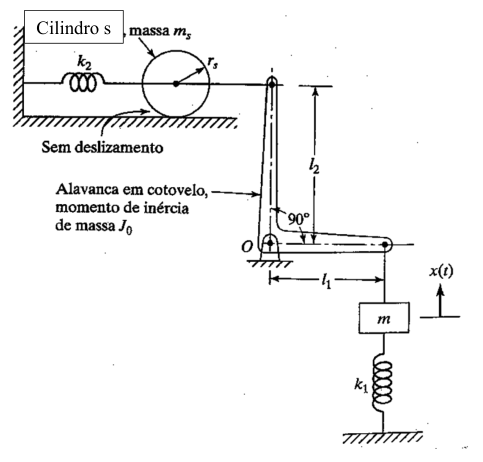
\includegraphics[width=0.4\textwidth]{imagens/lista_3_questao_1.png}
    %\caption{questao1}
    \label{fig:questao1}
\end{figure}

\resol
As equações que regem o sistema são:
\[
    E_c = \frac{1}{2}m_{s}\cdot {\dot{x}_{s}^2} + \frac{1}{2}J_{s}\theta_{s}^2 + \frac{1}{2}J_0\theta_{0}^2 + \frac{1}{2}m\cdot \dot{x}^2
\]
\[
    E = \frac{1}{2}m_{eq}\cdot \dot{x}_{eq}^2 = \frac{1}{2}m_{eq}\cdot \dot{x}_s^2
\]

Encontrando termos em comum para substituir nas equações\ldots

$\dot{x}_s = \dot{\theta}_s \cdot r_s \to \dot{\theta}_s = \frac{\dot{x}_s}{r_s}$

Velocidade angular em $\dot{\theta}_0$:
\[
    \theta_0 = \frac{\dot{x}_s}{l_2}
\]
\[
    \dot x = \theta_0 \cdot l_1 \to \dot x = \frac{\dot{x}_s}{l_1}
\]
Substituindo na equação principal, temos:

    \begin{align*}
        E_c = &\frac{1}{2}m_s\cdot \dot{x}_s^2 + \frac{1}{2}J_s\cdot \left(
    \frac{\dot{x}_s}{r_s} \right)^2 +\\ &\frac{1}{2}J_0\cdot \left( \frac{\dot {x}_s}{l_2} \right)^2 + \frac{1}{2}\cdot \left( \frac{\dot {x}_s\cdot l_1}{l_2} \right)^2
    \end{align*}

Multiplicando ambos os lados da equação por 2 e dividindo por $\dot{x}_s$
cancela-se esses termos obtendo a equação:

 \[
     m_{eq}= m_s + J_s\cdot \frac{1}{r_s^2}+ J_0\cdot \frac{1}{{l_2}^2} + \frac{{l_1}^{2}}{{l_2}^{2}}
\]


\subsection{Questão 2}
Analisando a figura abaixo, que representa um sistema de acionamento de válvula
de um motor de combustão interna, encontre a massa equivalente para o sistema;
tendo como referência a vareta.
\begin{figure}[ht]
    \centering
    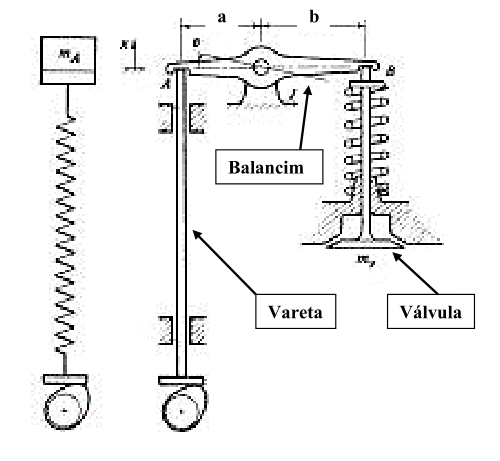
\includegraphics[width=0.4\textwidth]{imagens/lista_3_questao_2.png}
    %\caption{}
    \label{fig:questao2}
\end{figure}
\resol

\begin{equation}\label{eq:lista_3_questao_2_energia}
    T = \frac{1}{2}\cdot m\cdot \dot{x}^2 + \frac{1}{2} J_b \theta_b^2 + \frac{1}{2} m_v\cdot \dot{x}_v^2
\end{equation}

\[
    \dot{\theta}_b = \frac{\dot x}{a}\quad ; \dot\theta_b= \frac{\dot x_v}{b}
\]
Igualando uma com a outra e isolando $\dot x_v$ :
\begin{equation}\label{eq:lista_3_questao_2_teta}
 \dot x_v=\frac{\dot x}{a}\cdot b
\end{equation}

Substituindo (\ref{eq:lista_3_questao_2_teta}) em
(\ref{eq:lista_3_questao_2_energia}):
\[
    \frac{1}{2}\cdot m \cdot \dot x^2 + \frac{1}{2}J_b\cdot \left( \frac{\dot x}{a} \right)^2 + \frac{1}{2}m_v \left(\frac{\dot x \cdot b}{a}  \right)^2
\]
\[
    \cancel{\frac{1}{2}}m_{eq}\cdot\bcancel{\dot x^2} = \cancel{\frac{1}{2}}m\cdot\bcancel{\dot x^2} + \cancel{\frac{1}{2}}J_b\cdot \left( \frac{\bcancel{\dot x}}{a} \right)^2 + \cancel{\frac{1}{2}}m_v \cdot \left( \frac{\bcancel{\dot x}b}{a} \right)^2
\]

\[
m_{eq}= m + \frac{J_b}{a^2} + m_v\cdot \frac{b^2}{a^2}
\]
